% --
% mfcc

\section{Mel Frequency Cepstral Coefficients}\label{sec:signal_mfcc}
This section describes why MFCCs are appropriate features for speech recognition tasks, how they are calculated, and how they can be enhanced.
Moreover, a normalization technique for an improved visualization of MFCCs is presented.


% --
% idea

\subsection{The Idea}
The processing scheme of MFCCs \cite{Davis1980MFCC} is as follows:
Raw audio samples are transformed into the frequency domain with the STFT.
Afterwards the power spectrum of the STFT is computed and segmented into frequency bands through equidistantly spaced triangular window functions on the Mel scale.
The Mel scale was developed in psycho-acoustic experiments, where researchers learned that high frequency sounds (above approximately \SI{500}{\hertz}) are perceived lower than they actually are.
Consequently, the Mel scale shares a non-linear relationship with the frequency scale and is further described in \rsec{signal_mfcc_pipeline}.
Note that the Mel scale is suited to the perception of pitch and that separating the frequency space into equidistant Mel bands is therefore reasonable.

Another important processing step is the logarithmic scaling of the power spectrum's value space motivated by the logarithmic perception of loudness of humans.
The last step is to apply the Discrete Cosine Transform (DCT) to the individual filter bands.
Note that the DCT is a widely used technique in image processing and compression.
In the applications of MFCCs, the DCT is applied as decorrelation process of the filter bands.

The mentioned processing steps to compute MFCCs seem rather complicated but are nothing more than consecutive steps of appropriate scaling and data compression.


% --
% processing pipeline

\subsection{Processing Pipeline in Detail}\label{sec:signal_mfcc_pipeline}
The frequency spectrum is separated into filter bands through triangular window functions.
Those window functions are equidistantly placed onto the Mel scale and therefore result in a varying number of frequency bins in the frequency scale for each window.
The lower frequency bands receive fewer frequency bins than the higher frequency bands.
Sometimes the height of the individual triangular windows is scaled down such that the effect of unequal amounts frequency bins is equalized.
However, high frequency signals usually carry less energy so that this scaling is in most cases neglected or not preferred.

The Mel - frequency relation can be approximated by the function
\begin{equation}\label{eq:signal_mfcc_mel}
  m(f) = 2595 \cdot \log_{10} \left(1 + \frac{f}{700} \right),
\end{equation}
where $m$ is the result in Mel scale as function of the frequency $f$.
The Mel scale plotted against the frequency scale is illustrated in \rfig{signal_mfcc_mel_scale}.
\begin{figure}[!ht]
  \centering
  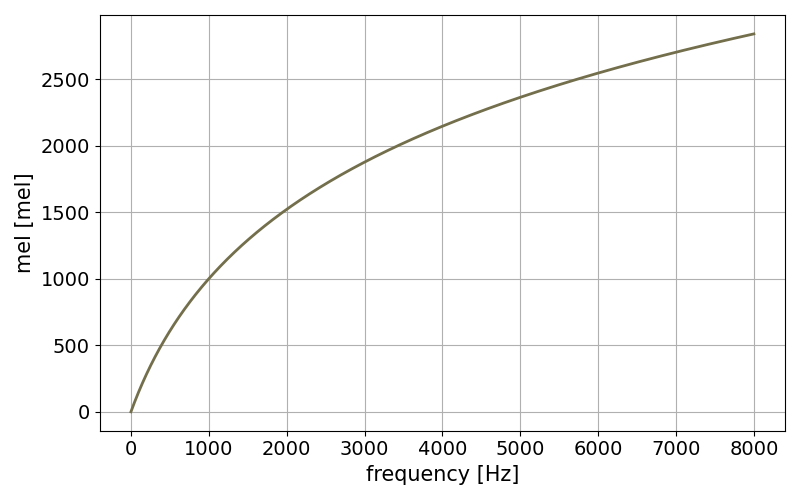
\includegraphics[width=0.48\textwidth]{./3_signal/figs/signal_mfcc_mel_scale.png}
  \caption{Mel scale as function of the frequency in a range of [0, \SI{8}{\kilo\hertz}].}
  \label{fig:signal_mfcc_mel_scale}
\end{figure}
\FloatBarrier
\noindent
\rfig{filter_bands} provides the equidistantly spaced triangular window functions on the Mel scale and their representation on the frequency axis.
\begin{figure}[!ht]
  \centering
  \subfigure[Mel space]{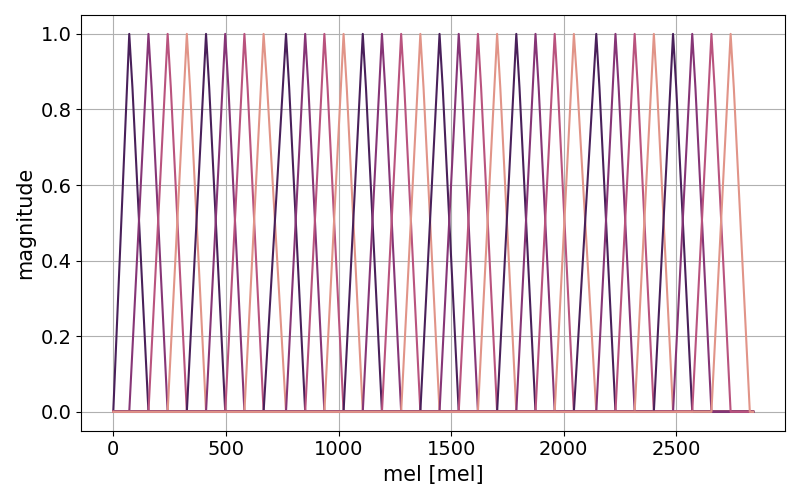
\includegraphics[width=0.48\textwidth]{./3_signal/figs/signal_mfcc_weights_mel.png}}
  \quad
  \subfigure[frequency space]{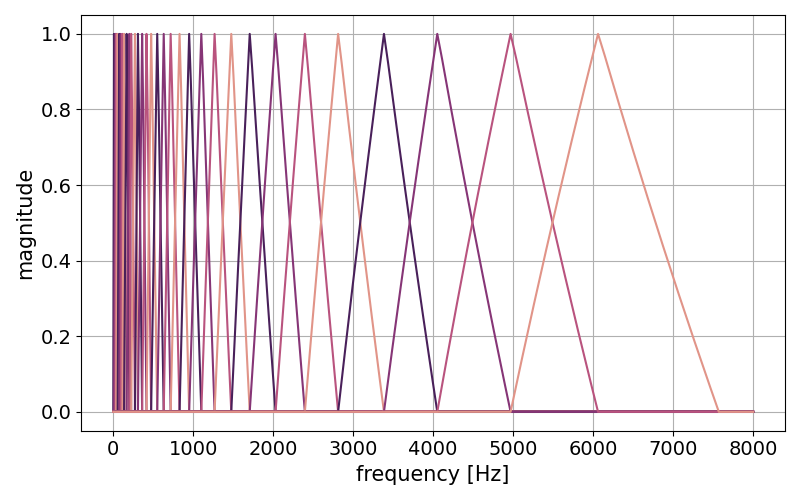
\includegraphics[width=0.48\textwidth]{./3_signal/figs/signal_mfcc_weights_f.png}}
  \caption{Equidistant Mel filter bands with a total number of 32 bands.}
  \label{fig:filter_bands}
\end{figure}
\FloatBarrier
\noindent
Note that the maximum frequency of the filter bands is $\SI{8}{\kilo\hertz}$ corresponding to the half of the sampling frequency $f_s = \SI{16}{\kilo\hertz}$.
The creation of those filter bands is not described mathematically because the graphical showcase is much more intuitive and easier to comprehend.
For further calculations, those filter bands are collected in a weight matrix $W_m \in \R^{B \times K}$, where $B$ is the amount of filter bands and $K$ the amount of frequency bins of the DFT transformed input signal.

% dct
The DCT is very similar to the Fourier transform and projects the input signal to a set of sinusoidal basis functions. 
However, the transformed signal remains real instead of complex valued.
Different types of DCT formulations exist but most commonly the \enquote{type 2} DCT is applied by its following definition:
\begin{equation}\label{eq:signal_mfcc_dct}
  \hat{x}[c] = \sum_{n=0}^{N-1} x[n] \cos{\left[ \frac{\pi}{N} \left( n + \frac{1}{2} \right) c \right]},
\end{equation}
where $c$ is the cepstral index and $n$ the sample index of a signal vector $\bm{x} \in \R^N$ with total length of $N$.
Again this can be conveniently written in matrix notation with a total number of $C$ cepstral coefficients as
\begin{equation}\label{eq:signal_mfcc_dct_matrix}
  \begin{aligned}
    \hat{\bm{x}} = \mathcal{D} \bm{x} \quad \mathrm{with} 
    \quad &\mathcal{D}[c, n] = \cos{\left[ \frac{\pi}{N} \left( n + \frac{1}{2} \right) c  \right]},\\
    &c, n = (0, 1, \dots, C - 1), (0, 1, \dots, N - 1),
  \end{aligned}
\end{equation}
where $\mathcal{D} \in \R^{C \times N}$ is the DCT matrix and $\hat{\bm{x}} \in \R^C$ the transformed signal.
The DCT basis functions are illustrated in \rfig{signal_mfcc_dct} in two different color schemes.
\begin{figure}[!ht]
  \centering
  \subfigure[continuous color scheme]{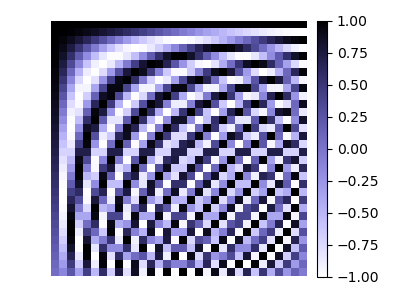
\includegraphics[width=0.35\textwidth]{./3_signal/figs/signal_mfcc_dct.png}}
  \qquad
  \subfigure[diverging color scheme]{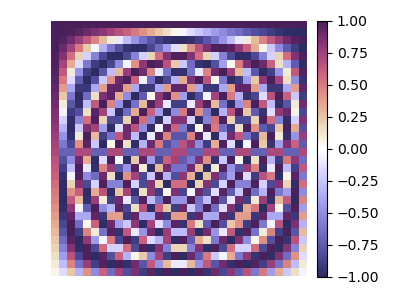
\includegraphics[width=0.35\textwidth]{./3_signal/figs/signal_mfcc_dct-div.png}}
  \caption{DCT matrix with 32 basis functions illustrated with a continuous and a diverging color scheme. The rows are the cepstral coefficients and the columns represent the length of the signal for transformation.}
  \label{fig:signal_mfcc_dct}
\end{figure}
\FloatBarrier
\noindent
The MFCCs $U \in \R^{C \times M}$ are calculated from the power spectrum of the STFT $P \in \R^{K \times M}$, the filter band weights collected in the matrix $W_m \in \R^{B \times K}$, and the DCT transformation matrix $\mathcal{D} \in \R^{C \times B}$ by following equation:
\begin{equation}\label{eq:signal_mfcc_mfcc}
  U = \mathcal{D} \log{ \left( W_m   P \right) }.
\end{equation}
Note that the rows of $U$ represent the cepstral coefficients and the columns the frames (shifts of the analytical window by the hop size).
The required parameters for the computations of MFCCs are therefore the amount of filter bands $B$ and the amount of cepstral coefficients $C$.

Another important aspect is the visualization of MFCC features.
MFCCs computed as described above, are not well suited for visualization purposes because their individual coefficient's value space differs strongly from each other.
For example, the first coefficient is calculated as summation of all filter bands of the spectrogram and therefore equals an energy measure.
The other coefficients on the other hand, are differently weighted sum combinations of the filter bands.
Furthermore, the most of the energy in speech signals is located in the lower frequency bands, which impacts the value space of the coefficients with strongly weighted low frequency bands.
The differences in the value space lead to a problem in the visualization with a linear color scheme such that the changes of some coefficients cannot be presented properly.
A solution to this problem is to normalize the feature vectors over their frame dimension by
\begin{equation}\label{eq:signal_mfcc_norm}
  U[c, m] \gets \frac{U[c, m] + \vert \underset{m \in \mathcal{M}}{\min} \bm{u}_c \vert}{\norm{\bm{u}_c + \vert \underset{m \in \mathcal{M}}{\min} \bm{u}_c \vert}_\infty} \quad \forall \, c, m = (0, 1, \dots, C - 1), (0, 1, \dots, M - 1),
\end{equation}
where $c$ is the cepstral index, $m$ the frame (time) index, and $\bm{u}_c \in \R^M$ the individual MFCC coefficient vector over all frames $M$.
This equation results in a value space between $[0, 1]$ for each feature vector $\bm{u}_c$.
This normalization technique is denoted as \emph{frame-based normalization} and will be an important evaluation subject in the following sections.

A visualization of MFCC features with 32 filter bands, 32 cepstral coefficients, and frame-based normalization is shown in \rfig{signal_mfcc_showcase_mfcc32}.
\begin{figure}[!ht]
  \centering
    \subfigure[left]{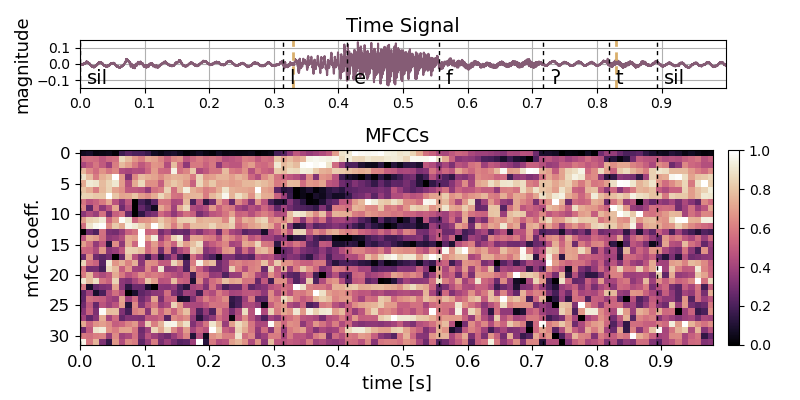
\includegraphics[width=0.45\textwidth]{./3_signal/figs/signal_mfcc_showcase_mfcc32_left0.png}}
    \subfigure[right]{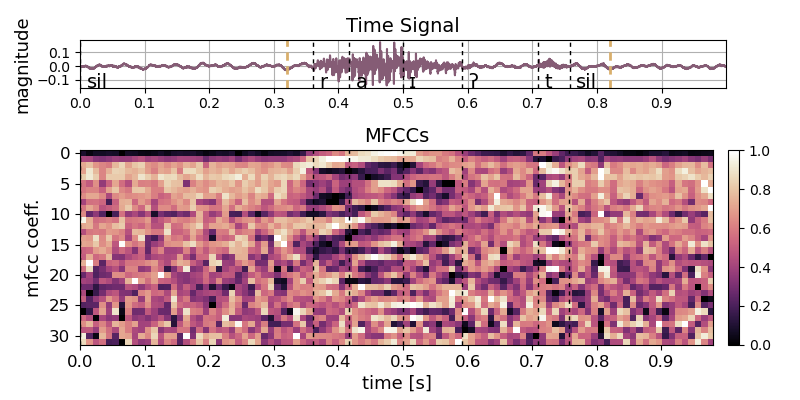
\includegraphics[width=0.45\textwidth]{./3_signal/figs/signal_mfcc_showcase_mfcc32_right0.png}}
    \subfigure[up]{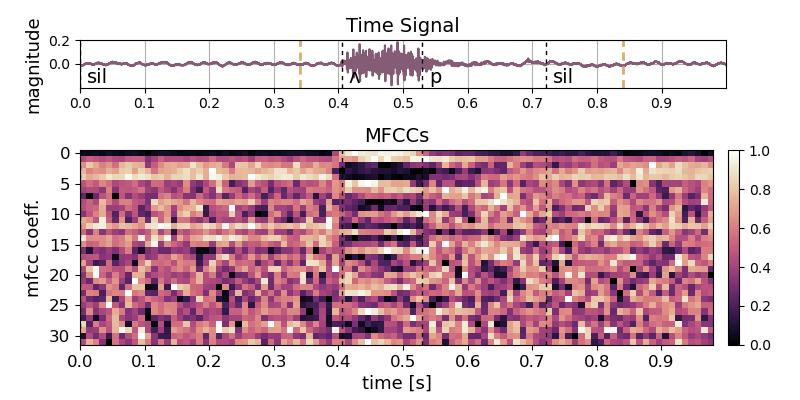
\includegraphics[width=0.45\textwidth]{./3_signal/figs/signal_mfcc_showcase_mfcc32_up0.png}}
    \subfigure[down]{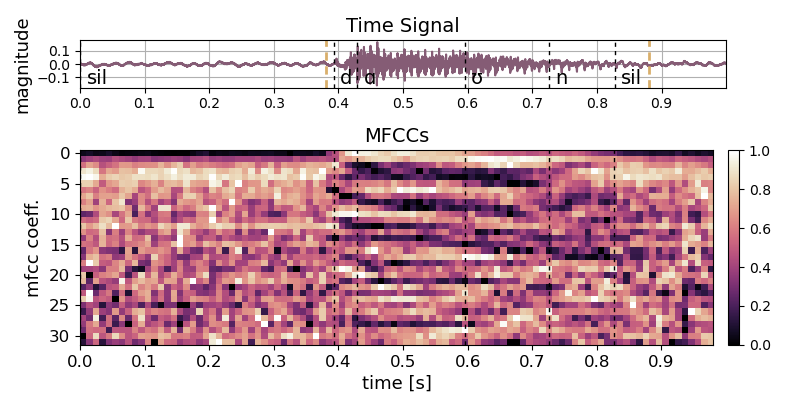
\includegraphics[width=0.45\textwidth]{./3_signal/figs/signal_mfcc_showcase_mfcc32_down0.png}}
    \subfigure[go]{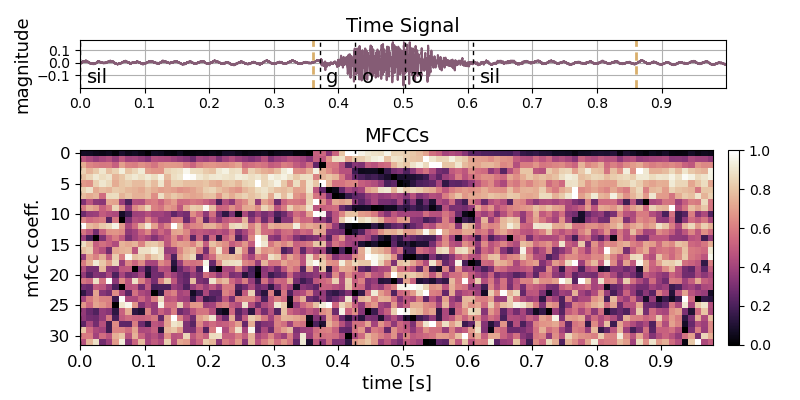
\includegraphics[width=0.45\textwidth]{./3_signal/figs/signal_mfcc_showcase_mfcc32_go0.png}}
  \caption{MFCC with 32 filter bands and 32 cepstral coefficients visualized with frame-based normalization.}
  \label{fig:signal_mfcc_showcase_mfcc32}
\end{figure}
\FloatBarrier
\noindent
The frame-based normalization is an interesting technique that improves the visualization of MFCC features.
Nevertheless, this normalization technique can be critical. 
A normalization that operates only in one dimension changes valuable structures within the other dimensions, and it cannot be answered yet, whether this is a problem for the classification task in the later sections.
One more research question arises here: Is it possible to use frame-based normalized MFCC features as input to neural network models and what is the impact on the classification accuracy?


% --
% enhancement

\subsection{MFCC Feature Usage and Enhancement}\label{sec:signal_mfcc_enhancement}
After MFCCs are computed by choosing the amount of filter bands $B$ and cepstral coefficients $C$, they can already be used as input features for neural networks.
The question arises, whether feature enhancements can improve the performance in classification.
The best practice applied in many papers, is to use $B=32$, $C=12$, compute derivatives of those 12 MFCCs, referred to as \emph{deltas} (first derivative regarding the frame dimension) and \emph{double deltas} (second derivative) and add \emph{energy vectors} of the 12 coefficients and each one of the deltas.
The deltas are computed as frame difference of the MFCCs by
\begin{equation}\label{eq:signal_mfcc_delta}
  \Delta u_c[m] = \frac{u_c[m - 1] + u_c[m + 1]}{2},
\end{equation}
where $u_c[m]$ is the c-th MFCC coefficient at frame $m$, where $m = 0, 1, \dots, M - 1$ is the frame index of a total number of $M$ frames.
Note that the computation of the deltas at the edges $m=0$ and $m=M - 1$ is not possible and that the same value is obtained from the neighbor at this specific locations.
The second derivative of MFCC features, known as double deltas, are the frame differences of the deltas and likewise computed as in \req{signal_mfcc_delta}.
Another enhancement is the computation of an energy feature vector $\bm{e} \in \R^M$ that can be computed with
\begin{equation}
  e[m] = \bm{u}[m]^T \bm{u}[m]
\end{equation}
for all frames $m$.
The same energy computation may also be applied to the deltas and double deltas.

A concatenation of all features vectors and their enhancements into a single feature matrix is usually performed by simply stacking the MFCCs, their deltas, double deltas, and energy vectors at top of each other.
In this thesis the stacking of features and enhancements is done in following constellation:
\begin{enumerate}
    \item 12 MFCCs,
    \item 1 energy feature of the 12 MFCCs,
    \item 12 deltas,
    \item 1 energy feature vector of the 12 deltas,
    \item 12 double deltas, and
    \item 1 energy feature vector of the 12 double deltas,
\end{enumerate}
which sums up to a 39-dimensional feature vector, referred to as MFCC-39.
\rfig{signal_mfcc_showcase_mfcc39} visualizes the MFCC-39 from the showcase examples.
\begin{figure}[!ht]
  \centering
    \subfigure[left]{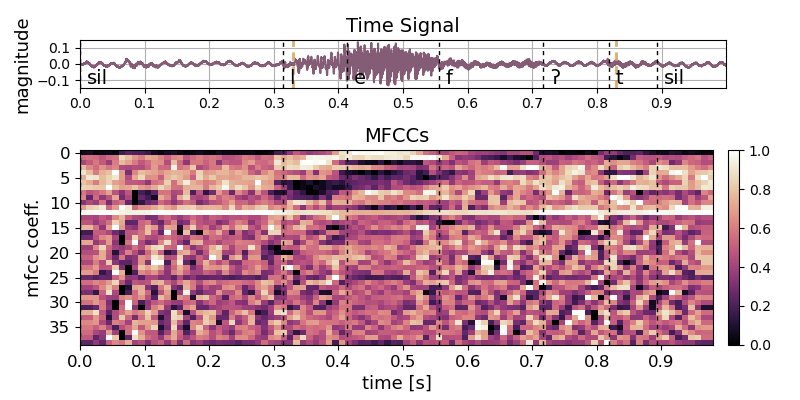
\includegraphics[width=0.45\textwidth]{./3_signal/figs/signal_mfcc_showcase_mfcc39_left0.png}}
    \subfigure[right]{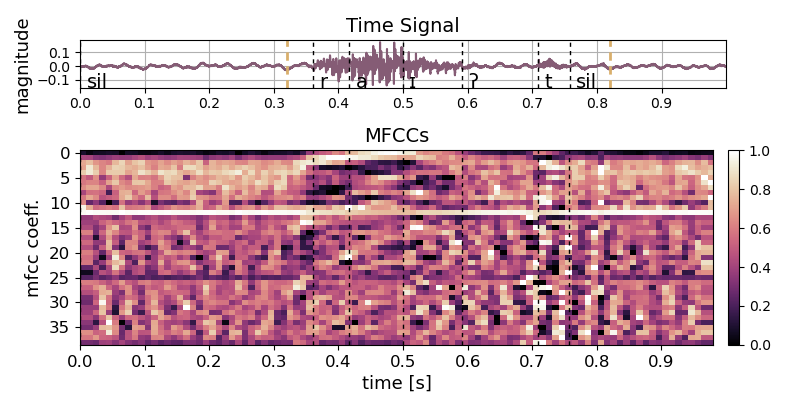
\includegraphics[width=0.45\textwidth]{./3_signal/figs/signal_mfcc_showcase_mfcc39_right0.png}}
    \subfigure[up]{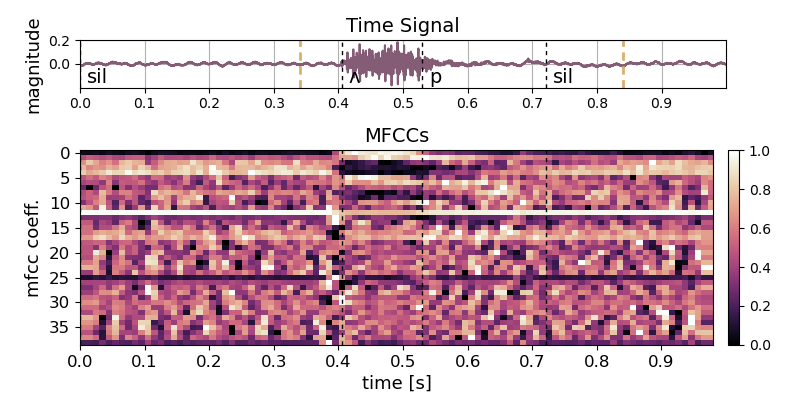
\includegraphics[width=0.45\textwidth]{./3_signal/figs/signal_mfcc_showcase_mfcc39_up0.png}}
    \subfigure[down]{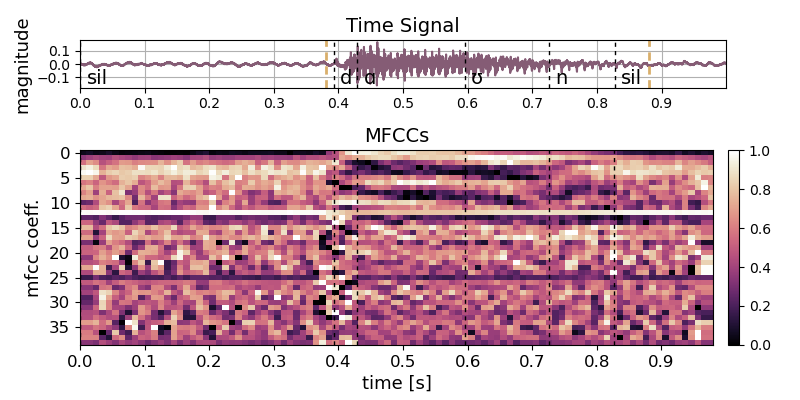
\includegraphics[width=0.45\textwidth]{./3_signal/figs/signal_mfcc_showcase_mfcc39_down0.png}}
    \subfigure[go]{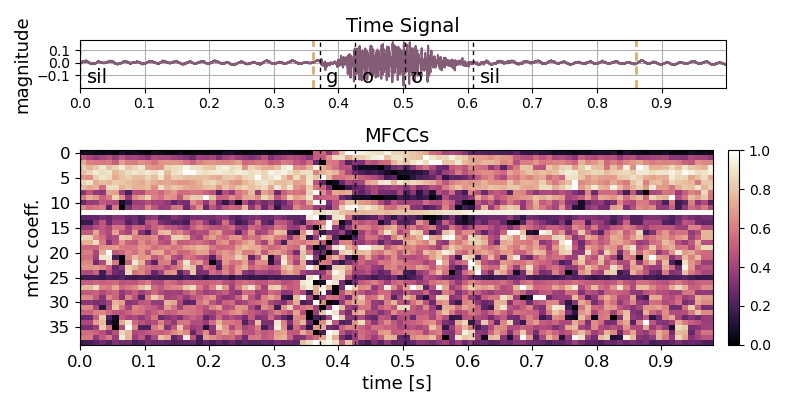
\includegraphics[width=0.45\textwidth]{./3_signal/figs/signal_mfcc_showcase_mfcc39_go0.png}}
  \caption{MFCCs extracted from the showcase examples with 32 filter bands and 12 cepstral coefficients, deltas, double deltas, and energy vector visualized with frame-based normalization.}
  \label{fig:signal_mfcc_showcase_mfcc39}
\end{figure}
\FloatBarrier
\noindent


% --
% energy consumption

\subsection{Computational Complexity}\label{sec:signal_mfcc_complexity}
The energy consumption is related to the computational complexity but much harder to define as it depends on many parameters and actual hardware implementations, which is especially relevant to handheld devices.
In this thesis however, it is sufficient to determine the computational complexity evaluated on the amount of operations required to process a specific computational task, such as the feature extraction of MFCCs.
The amount of operations is composed of the total number of additions and multiplications that are required to fulfill this specific task.
Further, it provides a comparison to the benchmark models mentioned in \rsec{prev_kws_benchmark}.
The computational complexity for the extraction of MFCC features is the amount of operations required to process a \SI{1}{\second} time signal sampled with $f_s = \SI{16}{\kilo\hertz}$.
The extraction details of the MFCCs are collected in \rtab{signal_mfcc_extraction_params}.
\begin{table}[ht!]
\small
\begin{center}
\caption{Parameters for determining the computational complexity of the MFCC feature extraction process.}
\begin{tabular}{ M{7cm}  M{2.5cm} M{2.5cm}}
\toprule
\textbf{Parameter} & \textbf{Value} & \textbf{Sample Length} \\
\midrule
Length of a signal $n$ & \SI{1}{\second} & 16000 \\
Analytic window size $N$ & \SI{25}{\milli\second} & 400 \\
Hop size $h$ & \SI{10}{\milli\second} & 160\\
\midrule
Fourier coefficients $K$ & 400  & - \\
Number of filter bands $B$ & 32 & -\\
Number of cepstral coefficients $C$ & 12 & -\\
\bottomrule
\label{tab:signal_mfcc_extraction_params}
\end{tabular}
\end{center}
\vspace{-4mm}
\end{table}
\FloatBarrier
\noindent
The major components of the MFCC are, as described in \rsec{signal_mfcc_pipeline} and summarized in \req{signal_mfcc_mfcc}, the transformation to the STFT, the weighting with the filter bands, and the DCT transform.
The most costly component is of course the STFT, which again is composed of the DFT.
Note that the DFT uses complex multiplications and additions.
One complex multiplication equals to 4 real multiplication and 2 additions, so one complex multiplication consists of 6 operations.
For one complex addition, two real additions are necessary and equals therefore to 2 operations.
A general matrix multiplication with a vector $y = A \bm{x}$, where $A \in \R^{m \times n}$ and $\bm{x} \in \R^n$ is composed of $m \cdot n$ multiplications and $m \cdot (n - 1)$ additions.
Note that for simplicity the amount of additions is approximated by $m \cdot n$.

The amount of operations, denoted as $\mathcal{T(.)}$, for a trivial DFT transform of a windowed signal $\bm{x} \in \R^N$ with operator $\mathcal{F} \in \C^{K \times N}$, where $K$ is the number of Fourier coefficients and $N$ the sample length, is
\begin{equation}
  \mathcal{T}(\mathcal{F} \bm{x}) = 6 (N K) + 2 (N K).
\end{equation}
For example, using $N = K = 400$ results in $\mathcal{T}(\mathcal{F} \bm{x}) = \SI{1.28}{\mega\ops}$ for a single DFT.
This of course, are far too many operations to handle in real time systems.
Luckily, a more sophisticated Fourier transform can be applied by the Fast Fourier Transform (FFT) algorithm \cite{Brigham1967FFT}, which gives a linear complexity of
\begin{equation}
  \mathcal{T}(\mathcal{F} \bm{x}) = 6 (\mathcal{O}(N \cdot \log_2 N)) + 2 (\mathcal{O}(N \cdot \log_2 N)).
\end{equation}
The FFT has therefore roughly $\mathcal{T}(\mathcal{F} \bm{x}) = \SI{27.7}{\kilo\ops}$ and is a huge improvement to the trivial method.
The DFT is computed $M$ times, where $M$ is the total number of frames.
The total number of frames is calculated as already described in \req{signal_spec_hop} and results in $M = 98$ with the parameters in \rtab{signal_mfcc_extraction_params}.
To compute the whole STFT, $M$ is multiplied with the number of operations of each DFT, which results in approximately $\mathcal{T}(\tilde{X}) = \SI{2.71}{\mega\ops}$.
Note that only the half-band of each individual FFT is applicable because of the mirroring effect at $\frac{f_s}{2} = \SI{8}{\kilo\hertz}$.
The Fourier coefficients are therefore reduced to $K = 201$ for the following operations.

The computation of the power spectrum and the log scaling are disregarded so that two matrix multiplications remain:
$W_m P$ is a matrix multiplication of $\R^{B \times K}$ and $\R^{K \times M}$, which has $B K M$ real multiplications and approximately $B K M$ real additions, which give about $2 B K M = 2 \cdot 32 \cdot 201 \cdot 98 =  \SI{1.26}{\mega\ops}$.
Further, the resulting band weighted power spectrum $\R^{B \times M}$ is multiplied with the DCT operator representing a matrix of $\R^{C \times B}$ that gives $2 C B M = 2 \cdot 12 \cdot 32 \cdot 98 = \SI{75}{\kilo\ops}$.
Altogether the matrix multiplications are approximately $\SI{1.26}{\mega\ops} + \SI{75}{\kilo\ops} = \SI{1.34}{\mega\ops}$.

The summary of the estimated operations is listed in \rtab{signal_mfcc_operations}.
% --
% mfcc operations
\begin{table}[ht!]
\begin{center}
\caption{Approximated number operations needed to transform a \SI{1}{s} time signal to MFCCs with parameters listed in \rtab{signal_mfcc_extraction_params}.}
\begin{tabular}{ M{6cm}  M{4cm}}
\toprule
\textbf{Process} & \textbf{Approximated Number of Operations} \\
\midrule
Power spectrum & \SI{2.71}{\mega\ops}\\
Weighting with equidistant Mel bands & \SI{1.26}{\mega\ops}\\
DCT transform of the weighted power spectrum & \SI{75}{\kilo\ops}\\
\midrule
\textbf{Sum} & \SI{4.05}{\mega\ops}\\
\bottomrule
\label{tab:signal_mfcc_operations}
\end{tabular}
\end{center}
\vspace{-4mm}
\end{table}
\FloatBarrier
\noindent


% --
% critism

\subsection{Criticism}
MFCC are widely used for speech recognition tasks and perform very well upon them. 
However, the processing pipeline of MFCCs leave some disadvantages.
One disadvantage is, as already mentioned in \rsec{signal_mfcc_pipeline}, that MFCCs are not intended for visualization because of their broad value space of individual MFCC coefficients.
Another disadvantage is that MFCC are not directly invertible to raw audio samples because of the computation of the spectrogram and its Mel band weighting.
Inversion techniques for MFCCs exist, such as described in \cite{Boucheron2008}.
However, it is still very difficult to obtain good approximations when the phase information of the original signal is missing.
The inversion of MFCCs would have been very interesting when applied to the outputs of generative neural networks, such as GANs.